\section{Ferngesteuertes Modellauto}
\label{sec:Auto}
Das ferngesteuerte Modellauto, das verwendet wird, ist der Amewi Hammerhead. Dieses Modellauto ist im Größenverhältnis $\frac{1}{6}$ gebaut, daraus ergibt sich eine Länge von 658 \ac{mm}, eine Breite von 428 \ac{mm} und eine Höhe von 260 \ac{mm}. Der Motor des Autos ist ein bürstenloser Gleichstrommotor mit einer Drehzahl von 2350 Umdrehungen pro Minute pro Volt, dieser wird von einer \ac{ESC} mit Spannung versorgt, welche wie in Sektion \ref{subsec:tESC} beschrieben arbeitet. Dieser Motor ist über ein Getriebe mit einem Differential verbunden, welches wiederum über die Antriebswelle der Hinterräder mit diesen verbunden ist. Das gesamte Übersetzungsverhältnis beträgt $\frac{1}{12.8}$.
\begin{figure}[h]
\centering
\includegraphics[scale=0.1]{Getriebe.jpg}
\caption{Getriebe und Differential des Autos}
\label{fig:Getriebe}
\end{figure}
\\
Das Auto kommuniziert über eine 2.4 \ac{GHz} Funkanlage mit der Fernsteuerung, bei welcher es sich um eine GooLRC TG 3 handelt. Der Raddurchmesser der Vorderräder beträgt 153 \ac{mm}, der Raddurchmesser der Hinterräder beträgt 148 \ac{mm}, diese Information ist wichtig für die Berechnung der Geschwindigkeit anhand der Drehzahl. (beschrieben in Sektion \ref{subsec:RPMprogram}) Das Modellauto wiegt (ohne Modifikationen) ungefähr 12.5 Kilogramm, es werden zwei in Serie geschaltete Zeee 2S 7.4 \ac{V} 80C 5200 \ac{mAh} Lithium Polymer Akkus verwendet, um die \ac{ESC} mit Spannung zu versorgen. Für die Lenkung wird ein Lenkservo mit einem Drehmoment von 1500 \ac{Nmm} verwendet. In der Nähe des Servomotors ist zusätzlich ein Gyroskop angebracht, welches mit dem Servomotor arbeitet, um das Lenken des Fahrzeuges anfängerfreundlicher zu machen. Das Auto verfügt außerdem über Voll-Aluminium Öldruckstoßdämpfer, die Bodenplatte besteht aus Aluminium, der Rest der Karosserie ist aus Kunststoff gefertigt.
Da das Modellauto nicht Fabrikneu, sondern gebraucht ist und der Vorbesitzer in Sand-ähnlichem Terrain gefahren zu sein scheint, muss das Auto gesäubert werden. Dazu muss das Auto zerlegt werden, um alle verschmutzten Oberflächen aufzudecken und diese zu säubern. 
\begin{figure}[h]
\centering
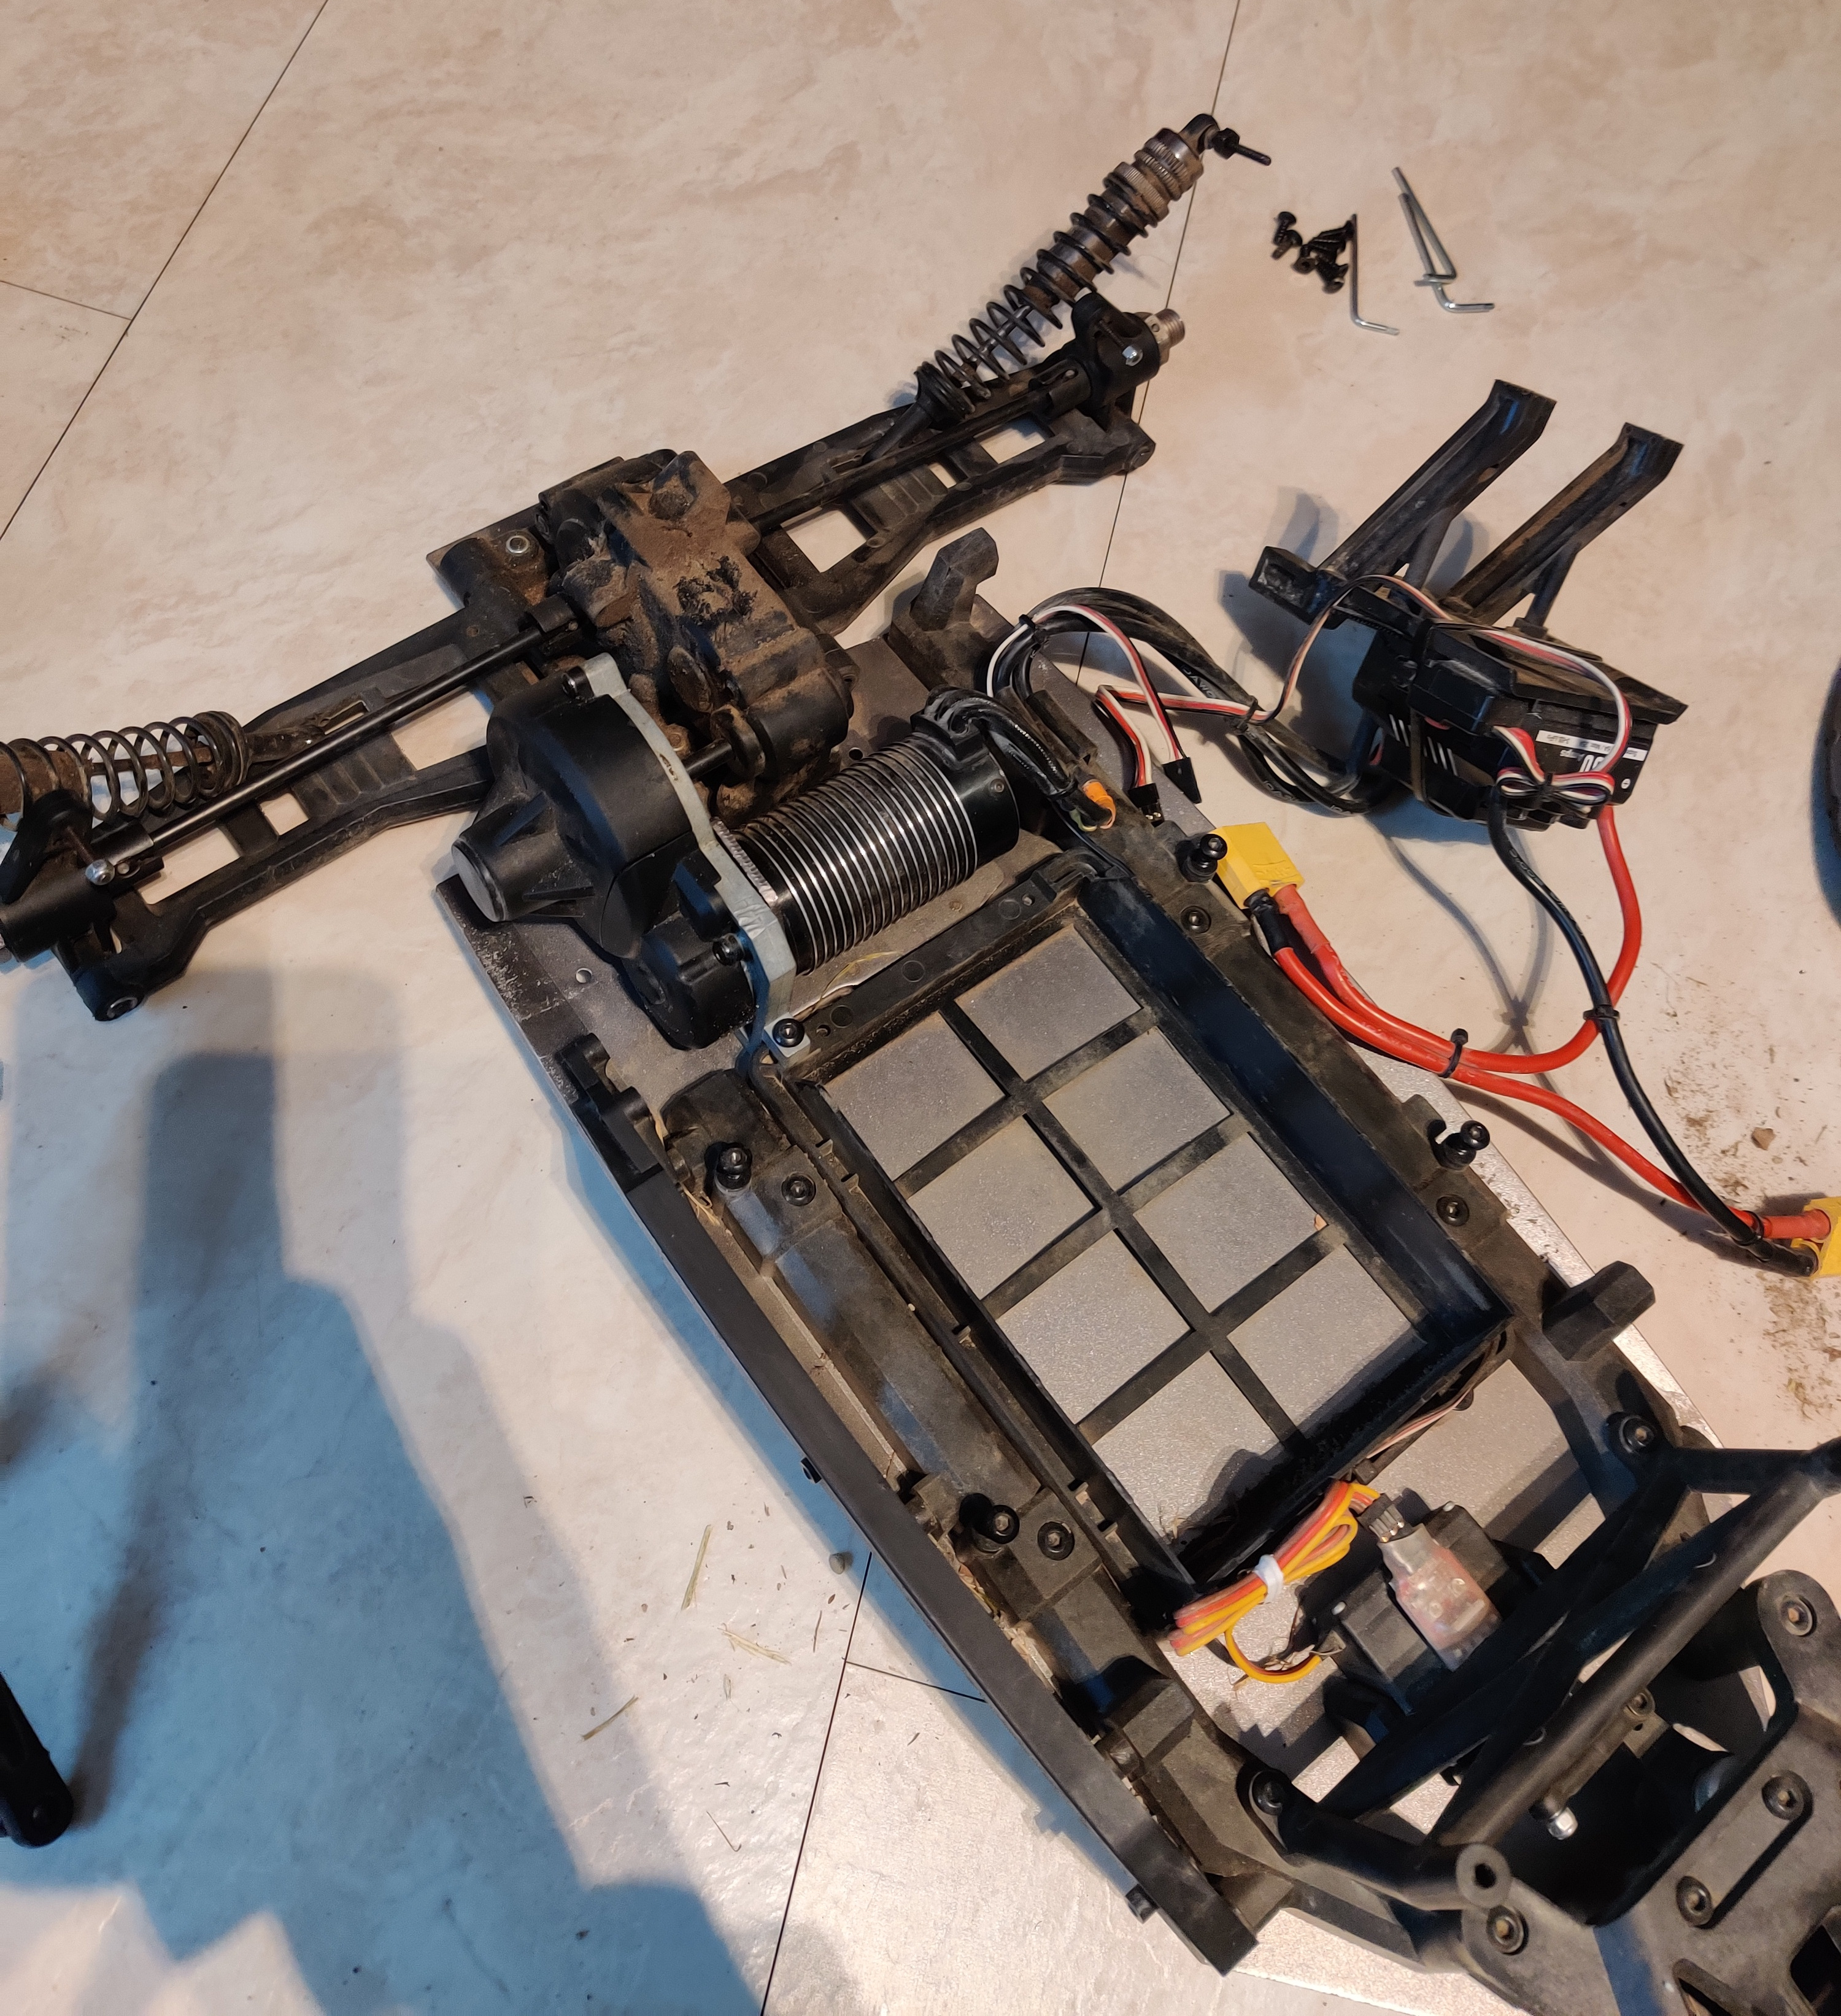
\includegraphics[scale=0.1]{AutoDreckig.jpg}
\caption{Verschmutztes Modellauto}
\label{fig:AutoDreckig}
\end{figure}